\section{Rejoindre le réseau}
\label{net:sec:joining}

\begin{figure*}
  \centering
  \subfloat[Un nœud \SPRAY rejoint un réseau.]
  [Le nœud $n_1$ contacte $n_2$ afin de rejoindre le réseau. $n_1$ ajoute
  $n_2$ à sa vue partielle.]
  {
\begin{tikzpicture}[scale=1.2]

  \newcommand\X{35pt};
  \newcommand\Y{15pt};

  \draw(-0.75*\X, 0pt); %% positioning
  \draw( 2.75*\X, 0pt); %% positioning

  \scriptsize
  \draw[->,dashed,very thick, color=darkblue](5+0*\X, 0*\Y) -- 
  node[anchor=south]{(a)}(-5+ 2*\X, 0*\Y);
  \draw[->] (-5+2*\X, 5pt) -- (5+\X, \Y);
  \draw[->] (-5+2*\X, 5pt) --  (5+\X, 2*\Y);
  \draw[->] (-5+2*\X, -5pt) -- (5+\X, -\Y);
  \draw[->] (-5+2*\X, -5pt) -- (5+\X, -2*\Y);

  \normalsize
  \draw[fill=white, very thick, draw=darkblue]
  (0*\X, 0*\Y) node{\DARKBLUE{$n_1$}} +(-5pt,-5pt) rectangle +(5pt,5pt);
  \draw[fill=white, very thick]
  (2*\X, 0*\Y) node{$n_2$} +(-5pt,-5pt) rectangle +(5pt,5pt);

  \draw[fill=white](1*\X,2*\Y) node{$n_6$} +(-5pt,-5pt) rectangle +(5pt,5pt);
  \draw[fill=white](1*\X,1*\Y) node{$n_5$} +(-5pt,-5pt) rectangle +(5pt,5pt);
  \draw[fill=white](1*\X,-1*\Y) node{$n_4$} +(-5pt,-5pt) rectangle +(5pt,5pt);
  \draw[fill=white](1*\X,-2*\Y) node{$n_3$} +(-5pt,-5pt) rectangle +(5pt,5pt);
  
\end{tikzpicture}}
  \hspace{40pt}
  \subfloat[Le contact annonce le nouvel arrivant.]
  [L'événement \textsc{onSubs}($n_1$) est déclanché en $n_2$ qui
  dissémine l'annonce.]
  {
\begin{tikzpicture}[scale=1.2]

  \newcommand\X{35pt};
  \newcommand\Y{15pt};

  \draw(-0.75*\X, 0pt); %% positioning
  \draw( 2.75*\X, 0pt); %% positioning

  \scriptsize
  \draw[->](5+0*\X, 0*\Y) -- (-5+ 2*\X, 0*\Y);
  \draw[->, very thick, color=darkblue] (-5+2*\X, 5pt) -- (5+\X, \Y);
  \draw[->, very thick, color=darkblue] (-5+2*\X, 5pt) --
  node[anchor=south west]{(b)} (5+\X, 2*\Y);
  \draw[->, very thick, color=darkblue] (-5+2*\X, -5pt) -- (5+\X, -\Y);
  \draw[->, very thick, color=darkblue] (-5+2*\X, -5pt) --
  node[anchor=north west]{(b)}(5+\X, -2*\Y);

  \normalsize
  \draw[fill=white]
  (0*\X, 0*\Y) node{$n_1$} +(-5pt,-5pt) rectangle +(5pt,5pt);
  \draw[fill=white, very thick, draw=darkblue]
  (2*\X, 0*\Y) node{\DARKBLUE{$n_2$}} +(-5pt,-5pt) rectangle +(5pt,5pt);

  \draw[fill=white, very thick]
  (1*\X,2*\Y) node{$n_6$} +(-5pt,-5pt) rectangle +(5pt,5pt);
  \draw[fill=white, very thick]
  (1*\X,1*\Y) node{$n_5$} +(-5pt,-5pt) rectangle +(5pt,5pt);
  \draw[fill=white, very thick]
  (1*\X,-1*\Y) node{$n_4$} +(-5pt,-5pt) rectangle +(5pt,5pt);
  \draw[fill=white, very thick]
  (1*\X,-2*\Y) node{$n_3$} +(-5pt,-5pt) rectangle +(5pt,5pt);

\end{tikzpicture}}
  \hspace{10pt}
  \subfloat[Les voisins du contact ajoute le nouvel arrivant.]
  [L'événement \textsc{onFwdSubs}($n_1$) est déclanché en $n_{3-6}$.
  Chacun de ces nœuds ajoute $n_1$ dans sa vue partielle.]
  {
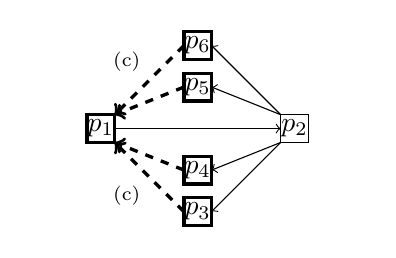
\begin{tikzpicture}[scale=1]

  \newcommand\X{35pt};
  \newcommand\Y{15pt};

  \draw(-0.75*\X, 0pt); %% positioning
  \draw( 2.75*\X, 0pt); %% positioning

  \scriptsize
  \draw[->](5+0*\X, 0*\Y) -- (-5+ 2*\X, 0*\Y);
  \draw[->] (-5+2*\X, 5pt) -- (5+\X, \Y);
  \draw[->] (-5+2*\X, 5pt) -- (5+\X, 2*\Y);
  \draw[->] (-5+2*\X, -5pt) -- (5+\X, -\Y);
  \draw[->] (-5+2*\X, -5pt) -- (5+\X, -2*\Y);

  \draw[->,dashed, very thick](-5+\X, 2*\Y) --
  node[anchor=south east]{(c)} ( 5pt,5pt);
  \draw[->,dashed, very thick](-5+\X, 1*\Y) -- ( 5pt,5pt);
  \draw[->,dashed, very thick](-5+\X, -1*\Y) -- ( 5pt,-5pt);
  \draw[->,dashed, very thick](-5+\X, -2*\Y) --
  node[anchor=north east]{(c)}( 5pt,-5pt);

  \normalsize
  \draw[fill=white, very thick]
  (0*\X, 0*\Y) node{$p_1$} +(-5pt,-5pt) rectangle +(5pt,5pt);
  \draw[fill=white]
  (2*\X, 0*\Y) node{$p_2$} +(-5pt,-5pt) rectangle +(5pt,5pt);

  \draw[fill=white, very thick]
  (1*\X,2*\Y) node{$p_6$} +(-5pt,-5pt) rectangle +(5pt,5pt);
  \draw[fill=white, very thick]
  (1*\X,1*\Y) node{$p_5$} +(-5pt,-5pt) rectangle +(5pt,5pt);
  \draw[fill=white, very thick]
  (1*\X,-1*\Y) node{$p_4$} +(-5pt,-5pt) rectangle +(5pt,5pt);
  \draw[fill=white, very thick]
  (1*\X,-2*\Y) node{$p_3$} +(-5pt,-5pt) rectangle +(5pt,5pt);
 

\end{tikzpicture}}
  \caption{\label{net:fig:joiningexample} Exemple de processus d'entrée dans
    le réseau de \SPRAY.}
\end{figure*}

Le processus d'entrée d'un nœud dans le réseau est, dans \SPRAY, la seule
manière d'introduire de nouveaux arcs. Afin de répondre à la première partie de
l'énoncé du problème~\ref{net:problem:properties}, ce nombre d'arcs doit
augmenter logarithmiquement comparé à la taille du réseau. Tout comme dans
\SCAMP, nous supposons que chacuns des nœuds respecte cette contrainte. Dès
lors, ces derniers utilisent cette supposition afin de propager l'adresse
logique du nouvel arrivant. L'algorithme~\ref{net:algo:joining} décrit la façon
dont le contact propage l'annonce à son voisinage où elle est directement
intégrée à leur vue partielle. En définitive, le nombre d'arcs dans le réseau
augmente de $1 + \ln |\mathcal{N}|$ et ce, seulement en utilisant des
interactions de voisin à voisin. Globalement, cela correspond à une augmentation
de l'ordre de $|\mathcal{N}| \ln |\mathcal{N}|$ arcs, similaire au seuil de
connexité exigé par les graphes aléatoires~\cite{erdos1959random}.

\begin{algorithm}[h]

\small
\algrenewcommand{\algorithmiccomment}[1]{\hskip2em$\rhd$ #1}

\newcommand{\comment}[1]{$\rhd$ #1}


\algblockdefx[initially]{initially}{endInitially}
  [0] {\textbf{INITIALLY:}} 

\algblockdefx[pas]{pas}{endPas}
  [0] {\textbf{EVENTS:}}

\newcommand{\LINEFOR}[2]{%
  \algorithmicfor\ {#1}\ \algorithmicdo\ {#2} %
  }

\newcommand{\LINEIFTHEN}[2]{%
  \algorithmicif\ {#1}\ \algorithmicthen\ {#2} %
  }

\newcommand{\INDSTATE}[1][1]{\State\hspace{\algorithmicindent}}

\begin{algorithmic}[1]
  \Statex
  \initially
    \State $\mathcal{P} \leftarrow \varnothing$;
    \hfill \comment{the partial view is a multiset}
    \State $p$ ; \hfill \comment{identity of the local peer}
  \endInitially
  
  \pas
  \Function{onSubs}{$o$} \hfill \comment{$o: origin$}
    \State \LINEFOR{\textbf{each} $\langle q,\,\_\, \rangle \in\mathcal{P}$}
    {$sendTo(q,\, 'fwdSubs',\, o)$;} \label{line:multicast}
    \EndFunction
    \Statex
    \Function{onFwdSubs}{$o$} \hfill \comment{$o: origin$}
    \State $\mathcal{P} \leftarrow
    \mathcal{P}\uplus \left\{\langle o,\, 0 \rangle\right\}$;
    \EndFunction
  \endPas
  
\end{algorithmic}

\caption{\label{net:algo:joining}The joining protocol of \SPRAY.}
\end{algorithm}

L'algorithme~\ref{net:algo:joining} présente les instructions de \SPRAY
concernant l'entrée d'un nouveau nœud dans le réseau. La vue partielle est un
multiensemble de couples $\langle n,\, age\rangle$ qui associe à chaque voisin
$n$ son âge dans la vue partielle $age$. Ce multiensemble permet de gérer les
doublons. Ces doublons sont généralement perçus négativement du fait de la
redondance d'information. Toutefois, ils nous sont nécessaire afin de ne pas en
perdre. L'âge joue le même rôle que dans \CYCLON, c'est à dire qu'il accélère la
suppression des nœuds avec lesquels il n'est plus possible de communiquer car
partis ou défaillant. L'événement \textsc{onSubs} est déclanché chaque fois qu'un
nœud rejoint le réseau via ce contact. Ce dernier distribue l'adresse logique du
nouvel arrivant à son voisinage, plusieurs fois aux doublons, et indépendament
de l'âge. L'événement \textsc{onFwdSubs} se déclanche lorsqu'un nœud reçoit la
redirection de l'adresse logique. Le nœud établit alors la connexion dont il
initialise l'âge à $0$.

La figure~\ref{net:fig:joiningexample} décrit un scénario où le pair $n_1$
contacte le pair $n_2$ afin de rejoindre le réseau composé de $\{n_2$, $n_3$,
$n_4$, $n_5$, $n_6\}$. Pour simplifier, la figure ne montre que les arcs
nouvellement introduits ainsi que les voisinages de $n_1$ et $n_2$. Le pair
$n_1$ ajoute directement $n_2$ dans sa vue partielle. Ce dernier redirige
l'adresse logique de $n_1$ à chacun de ses voisins.  Chacun de ces voisins
ajoute alors $n_1$ à leur vue partielle. Au total, \SPRAY établit 5
connexions. Le réseau en résultant est connexe.

Malheureusement, les vues partielles des derniers arrivant sont clairement
déséquilibrées comparé au reste du réseau. De ce fait, ils violent la première
condition de l'énoncé du problème~\ref{net:problem:properties}. Le processus de
mélange décrit dans la section suivante a pour objectif d'équilibrer les vues
partielles.


%%% Local Variables:
%%% mode: latex
%%% TeX-master: "../../paper"
%%% End:
